\documentclass[cn]{elegantbook}
\usepackage{amsmath,color}
\title{最优化方法:救命笔记}
\subtitle{献给还没复习的朋友们}
\author{Youwei Zhang}
\institute{天之智慧研究会}
\date{May 18,2022}
\version{1.0}
\extrainfo{各人自扫门前雪,休管他人瓦上霜。—— 我不同意}
\logo{logo}
\cover{cover}


\begin{document}
\maketitle

\pagestyle{empty}
\begin{center}
\textcolor[rgb]{0.33,0.33,1.00}{\huge \bf{1.牛顿法}}
\end{center}


\begin{algorithm}

给定控制误差$  \varepsilon>0 $.\\
Step 1 取初始点  $\boldsymbol{x}_{0} $, 令 $ k=0$ .\\
Step 2 计算$  \boldsymbol{g}_{\boldsymbol{k}} $.\\
Step 3 若 $ \left\|\boldsymbol{g}_{k}\right\| \leqslant \varepsilon $, 则  $\boldsymbol{x}^{*}=\boldsymbol{x}_{k} $, 停; 否则计算 $ \boldsymbol{G}_{k}$ , 并由 $G_kp_k=-g_k$  解 出  $\boldsymbol{p}_{k} $.\\
Step 4 令 $ \boldsymbol{x}_{k+1}=\boldsymbol{x}_{k}+\boldsymbol{p}_{k}, k=k+1 $, 转 Step  2 .
\end{algorithm}
\begin{exercisez}
试用牛顿(Newton)法求下列问题的最优解:
$$ \min f(x)=\frac{1}{2} x_{1}^{2}+\frac{3}{2} x_{2}^{2}-x_{1} x_{2}-2 x_{2} , $$

初始点  $x^{(0)}=(-1,-1)^{T} ;$
\end{exercisez}
\begin{solution}\\
$g(x)=\left(\begin{array}{c}
x_{1}-x_{2} \\
3x_{2}-x_{1}-2
\end{array}\right), G(x)=\left(\begin{array}{ll}
1 & -1 \\
-1 & 3
\end{array}\right)$正定\\
$x^{(0)}=(-1,-1)^{T},g_0=(0,-4)^{T},G_0=\left(\begin{array}{ll}
1 & -1 \\
-1 & 3
\end{array}\right)$\\
$\Rightarrow X^{(1)}=X^{(0)}-G^{-1} g_{0}=(1,1)^{T} ,\\ \text{此时,}  g_{1}=(0,0)^{T} , \text{故  } X^{*}=X^{(1)}=(1,1)^{T}, f^{*}=-1 .$
\end{solution}

\begin{exercisez}
试用牛顿(Newton)法求下列问题的最优解:

$$\min f(X)=x_{1}^{2}+2 x_{2}^{2}-2 x_{1} x_{2}-4 x_{1}, $$

$\text { 取初始点 } X^{(0)}=(1,1)^{T} \text {. }$

\end{exercisez}
\begin{solution}\\
$g(x)=\left(\begin{array}{c}
2x_{1}-2x_{2}-4 \\
4x_{2}-2x_{1}
\end{array}\right), G(x)=\left(\begin{array}{ll}
2 & -2 \\
-2 & 4
\end{array}\right)$正定\\
$x^{(0)}=(1,1)^{T},g_0=(-4,2)^{T},G_0=\left(\begin{array}{ll}
2 & -2 \\
-2 & 4
\end{array}\right)$\\
$\Rightarrow X^{(1)}=X^{(0)}-G^{-1} g_{0}=(4,2)^{T} ,\\ \text{此时,}  g_{1}=(0,0)^{T} , \text{故  } X^{*}=X^{(1)}=(4,2)^{T}, f^{*}=-8 .$
\end{solution}
\begin{note}
对于二次型函数,由于牛顿法的方向直指中心,且一步到位,能够一步走到极值点,所以求$X^{*}$的时候,直接令$g(x)=0$即可。
\end{note}

\newpage


\begin{center}
 \textcolor[rgb]{0.33,0.33,1.00}{\huge \bf{2.拟牛顿法}}
\end{center}

\begin{algorithm}
给定控制误差 $ \varepsilon $,\\
Step 1 给定初始点 $ \boldsymbol{x}_{0} $, 初始矩阵$  \boldsymbol{H}_{0}$  (通常取单位阵), 计算$  g_{0}$ , 令  $k=\mathbf{0} $.\\
Step 2 令  $\boldsymbol{p}_{k}=-\boldsymbol{H}_{k} \boldsymbol{g}_{k} $.\\
Step 3 由精确一维搜索确定步长  $\alpha_{k}$ ,

$\displaystyle f\left(x_{k}+\alpha_{k} p_{k}\right)=\min_{\alpha \geq 0} f\left(x_{k}+\alpha p_{k}\right) $.\\
Step 4 令 $ x_{k+1}=x_{k}+\alpha_{k} p_{k} $.\\
Step 5 若  $\left\|\boldsymbol{g}_{k+1}\right\| \leqslant \varepsilon$ , 则  $\boldsymbol{x}^{*}=\boldsymbol{x}_{k+1} $ 停; 否则令

$\boldsymbol{s}_{k}=\boldsymbol{x}_{k+1}-\boldsymbol{x}_{k},$ \quad $\boldsymbol{y}_{k}=\boldsymbol{g}_{k+1}-\boldsymbol{g}_{k} $.\\

Step 6 由 DFP 修正公式 $\boldsymbol{H}_{k+1}=\boldsymbol{H}_{k}-\frac{\boldsymbol{H}_{k} \boldsymbol{y}_{k} \boldsymbol{y}_{k}{ }^{\mathrm{T}} \boldsymbol{H}_{k}}{\boldsymbol{y}_{k}{ }^{\mathrm{T}} \boldsymbol{H}_{k} \boldsymbol{y}_{k}}+\frac{\boldsymbol{s}_{k} \boldsymbol{s}_{k}{ }^{\mathrm{T}}}{\boldsymbol{y}_{k}^{\mathrm{T}} \boldsymbol{s}_{k}}$得  $\boldsymbol{H}_{k+1} $. 令 $ k=k+1$ , 转 Step 2 .
\end{algorithm}
\begin{note}
\\
  1.确定初始点,行走方向(求这点的梯度$g_k$和$H_k$,方向$\boldsymbol{p}_{k}=-\boldsymbol{H}_{k} \boldsymbol{g}_{k}$) \\
  2.确定步长($\displaystyle \min_{\alpha \geq 0} f\left(x_{k}+\alpha p_{k}\right) $) \\
  3.走到下一点($ x_{k+1}=x_{k}+\alpha_{k} p_{k} $),再重复上述操作\\
\textcolor[rgb]{1.00,0.00,0.00}{\large 终止条件:}这一点的梯度$g_k=0$或很小的时候,就不要往下一个点走了,这点就为最优点.\\
\textcolor[rgb]{1.00,0.00,0.00}{\large $H_k$求解时的两个关键向量:}分别是两点的坐标差和梯度差\\
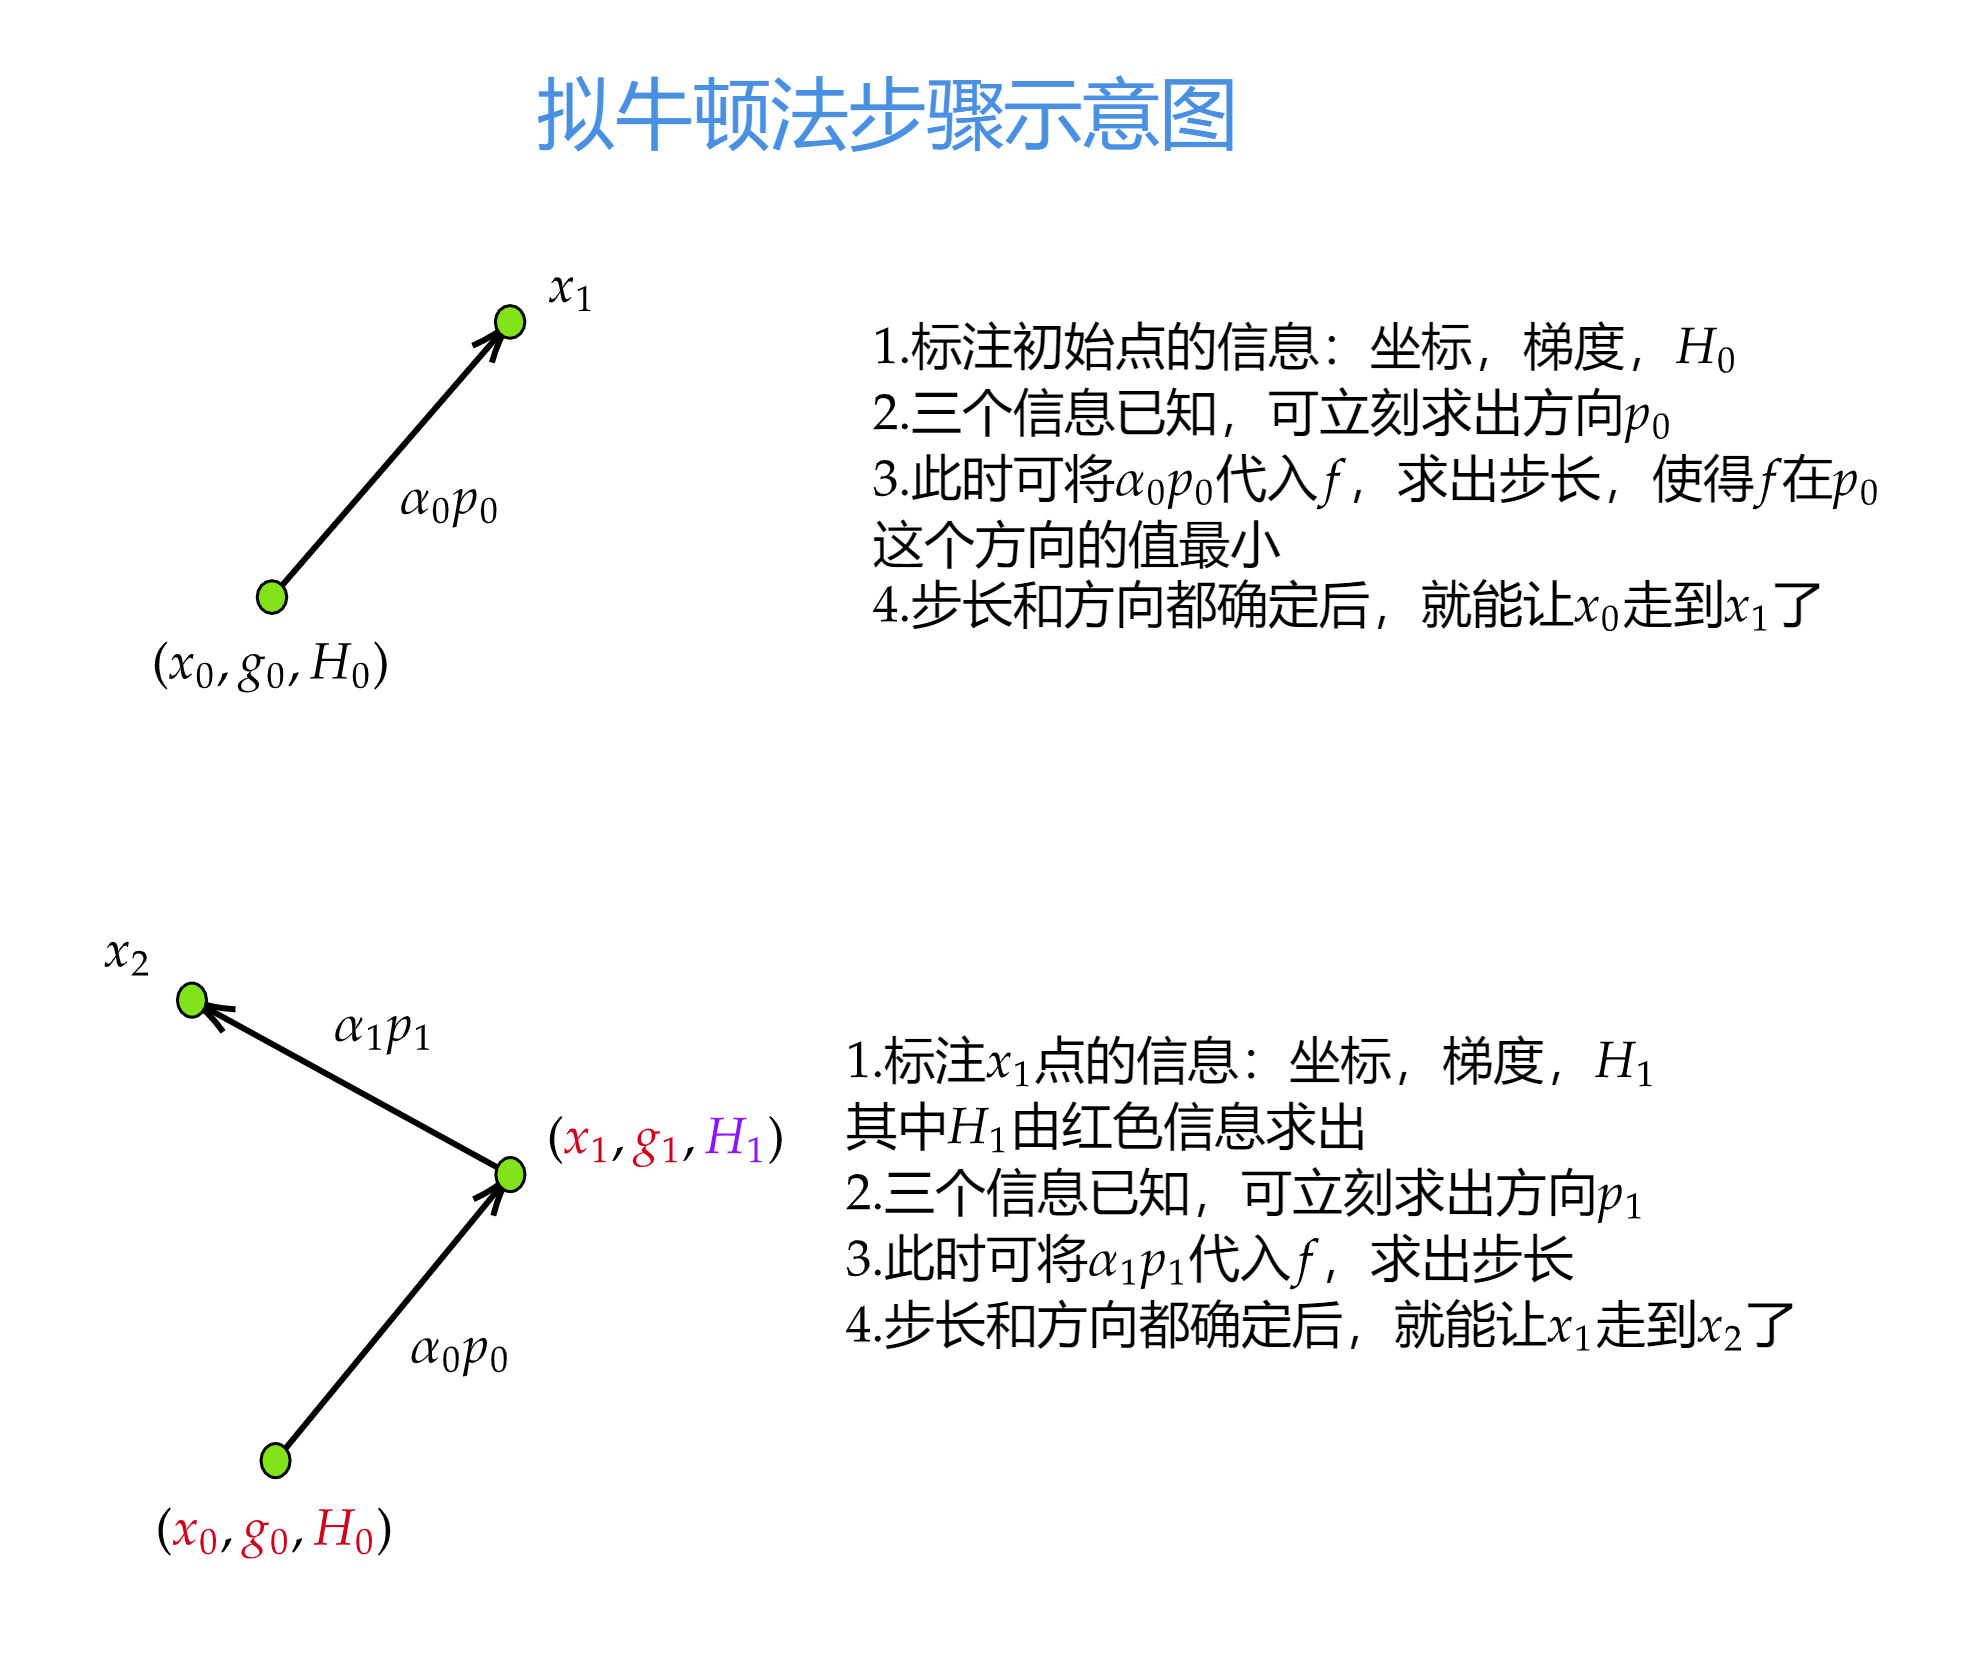
\includegraphics[width=0.85\textwidth]{fig1}
\end{note}
\begin{exercisez}
 用 DFP(变尺度)法求解下列无约束最优化问题:

$$\min f(x)=2 x_{1}^{2}+x_{2}^{2}+2 x_{1} x_{2}+x_{1}-x_{2} ;$$

取初始点$  x^{(0)}=(0,0)^{T}, H_{0}=E ;$
\end{exercisez}
\begin{solution}\\
$\nabla f(x)=\left(4 x_{1}+2 x_{2}+1,2 x_{2}+2 x_{1}-1\right),$
\vspace{5pt}

 \textcolor[rgb]{1.00,0.00,0.00}{\large 初始点信息:}
 $ x^{(0)}=(0,0)^{T}, g_{0}=(1,-1),
H_{0}=\left(\begin{array}{ll}
1 & \\
& 1
\end{array}\right),$
\vspace{5pt}

 \textcolor[rgb]{1.00,0.00,0.00}{\large 确定方向:}$ p_{0}=-H_{0} g_{0}=(-1,1)^{T},$
 \vspace{5pt}

 \textcolor[rgb]{1.00,0.00,0.00}{\large 确定步长:}$\displaystyle\min_{\lambda\geq 0} f(x^{(0)}+\lambda p_{0})=\min_{\lambda\geq 0}\lambda^{2}-2 \lambda, \varphi^{\prime}(\lambda)=2 \lambda-2=0, \text { 得 } \lambda_{0}=1, $
 \vspace{5pt}

 \textcolor[rgb]{1.00,0.00,0.00}{\large 走向下一点$x^{(1)}$}:$x^{(1)}=x^{(0)}+\lambda p_{0}=(-1,1)^{T},$
 \vspace{30pt}


 \textcolor[rgb]{0.00,0.50,1.00}{\large 新点$x^{(1)}$的信息:}$x^{(1)}=(-1,1)^{T},g_{1}=(-1,-1)^{T},H_1=$待求
 \vspace{5pt}

求解$H_1:$\\
$s_{0}=x^{(1)}-x^{(0)}=(-1,1)^{T}, y_{0}=g_{1}-g_{0}=(-2,0)^{T}, H_{1}=H_{0}+\frac{s_{0} s_{0}^{T}}{y_{0}^{T} s_{0}}-\frac{H_{0} y_{0} y_{0}^{T} H_{0}}{y_{0}^{T} H_{0} y_{0}} \\
=\left(\begin{array}{cc}
1 & 0 \\
0 & 1
\end{array}\right)+\frac{1}{2}\left(\begin{array}{cc}
1 & -1 \\
-1 & 1
\end{array}\right)-\frac{1}{4}\left(\begin{array}{cc}
4 & 0 \\
0 & 0
\end{array}\right)=\left(\begin{array}{cc}
1 / 2 & -1 / 2 \\
-1 / 2 & 3 / 2
\end{array}\right),$
\vspace{5pt}

 \textcolor[rgb]{0.00,0.50,1.00}{\large 确定$x^{(1)}$的行走方向:}$ p_{1}=-H_{1} g_{1}=\left(\begin{array}{c}
0 \\
-1
\end{array}\right),$
\vspace{5pt}

 \textcolor[rgb]{0.00,0.50,1.00}{\large 确定步长:}$\displaystyle\min_{\lambda\geq 0} f(x^{(1)}+\lambda p_{1})=\min_{\lambda\geq 0}\lambda^{2}-\lambda-1,
 \text { 得 } \lambda_{1}=\frac{1}{2},$
 \vspace{5pt}

   \textcolor[rgb]{0.00,0.50,1.00}{\large 走向下一点$x^{(2)}$:}$x^{(2)}=x^{(1)}+\lambda p_{1}=\left(-1, \frac{3}{2}\right)^{T},$
  \vspace{30pt}

  \textcolor[rgb]{1.00,0.00,0.00}{\large $x^{(2)}$的信息:}$x^{(2)}=\left(-1, \frac{3}{2}\right)^{T},g_{2}=(0,0)^{T}$,梯度为0,终止迭代.
  \vspace{5pt}

  所以极小点 $ x^{(2)}=(-1,3 / 2), f^{*}=-\frac{5}{4}.$

\end{solution}

\begin{exercisez}
 试用 DFP(变尺度)法, 求出 $ X^{(1)} $ 和变尺度矩阵 $ H_{1}$  以及搜索方向  $\boldsymbol{p}_{1} ,$
$$
\min f(X)=x_{1}^{2}+2 x_{2}^{2}-2 x_{1} x_{2}-4 x_{1},$$

$ \text { 取初始点 } X^{(0)}=(1,1)^{T}, H_{0}=E \text {. }
$
\end{exercisez}
\begin{solution}
过程如上,太麻烦了,自己写.
\end{solution}





\newpage
\begin{center}
 \textcolor[rgb]{0.33,0.33,1.00}{\huge \bf{3.共轭梯度法}}
\end{center}


\begin{algorithm}
给定控制误差$  \varepsilon$ .\\
Step 1 给定初始点 $ x_{1}, k=1 $.\\
Step 2 计算$  \boldsymbol{g}_{k}=\boldsymbol{g}\left(\boldsymbol{x}_{\mathbf{k}}\right) $.\\
Step 3 若$  \left\|\boldsymbol{g}_{k}\right\| \leqslant \varepsilon$ , 则  $\boldsymbol{x}^{*}=\boldsymbol{x}_{k}$  停;否则令
$$
\begin{array}{l}
\boldsymbol{p}_{k}=-\boldsymbol{g}_{k}+\beta_{k-1} \boldsymbol{p}_{k-1}, \\
\beta_{k-1}=\left\{\begin{array}{cl}
\frac{\boldsymbol{g}_{k}^{\mathrm{T}} \boldsymbol{g}_{k}}{\boldsymbol{g}_{k-1}^{\mathrm{T}} \boldsymbol{g}_{k-1}}, & \text { 当 } k>1 \text { 时, } \\
0, & \text { 当 } k=1 \text { 时. }
\end{array}\right.
\end{array}
$$
Step 4 由精确一维搜索确定步长$  \alpha_{k} $, 满足
$$
f\left(x_{k}+\alpha_{k} p_{k}\right)=\min _{a \geq 0} f\left(x_{k}+\alpha p_{k}\right) .
$$
Step 5 令  $\boldsymbol{x}_{k+1}=\boldsymbol{x}_{k}+\alpha_{k} \boldsymbol{p}_{k}, k=k+1$ , 转 Step 2 .
\end{algorithm}
\begin{note}
\\下面3句话不清楚什么意思不用管,直接看图即可.\\
  1.共轭梯度法核心是求一组共轭向量,也是G的特征向量,组成过渡矩阵P;在坐标变换$x=Py$下就是正交向量了,二次型的变量也解耦了。看二次型的等高线(椭圆)有,沿着共轭方向走,其实就是沿着变换后坐标系下的坐标轴方向走,由于变换后二次函数变量之间互不耦合,所以一维搜索下分别取极值后,就是最终的极值. \\
  2.共轭向量可以由已知点的梯度用类似"施密特共轭化"的方法求得,对于二次型函数,这个公式还可以简化 \\
  3.共轭梯度法也可以用来解实对称矩阵特征值,也就是解方程,参数量巨大也无所谓\\
  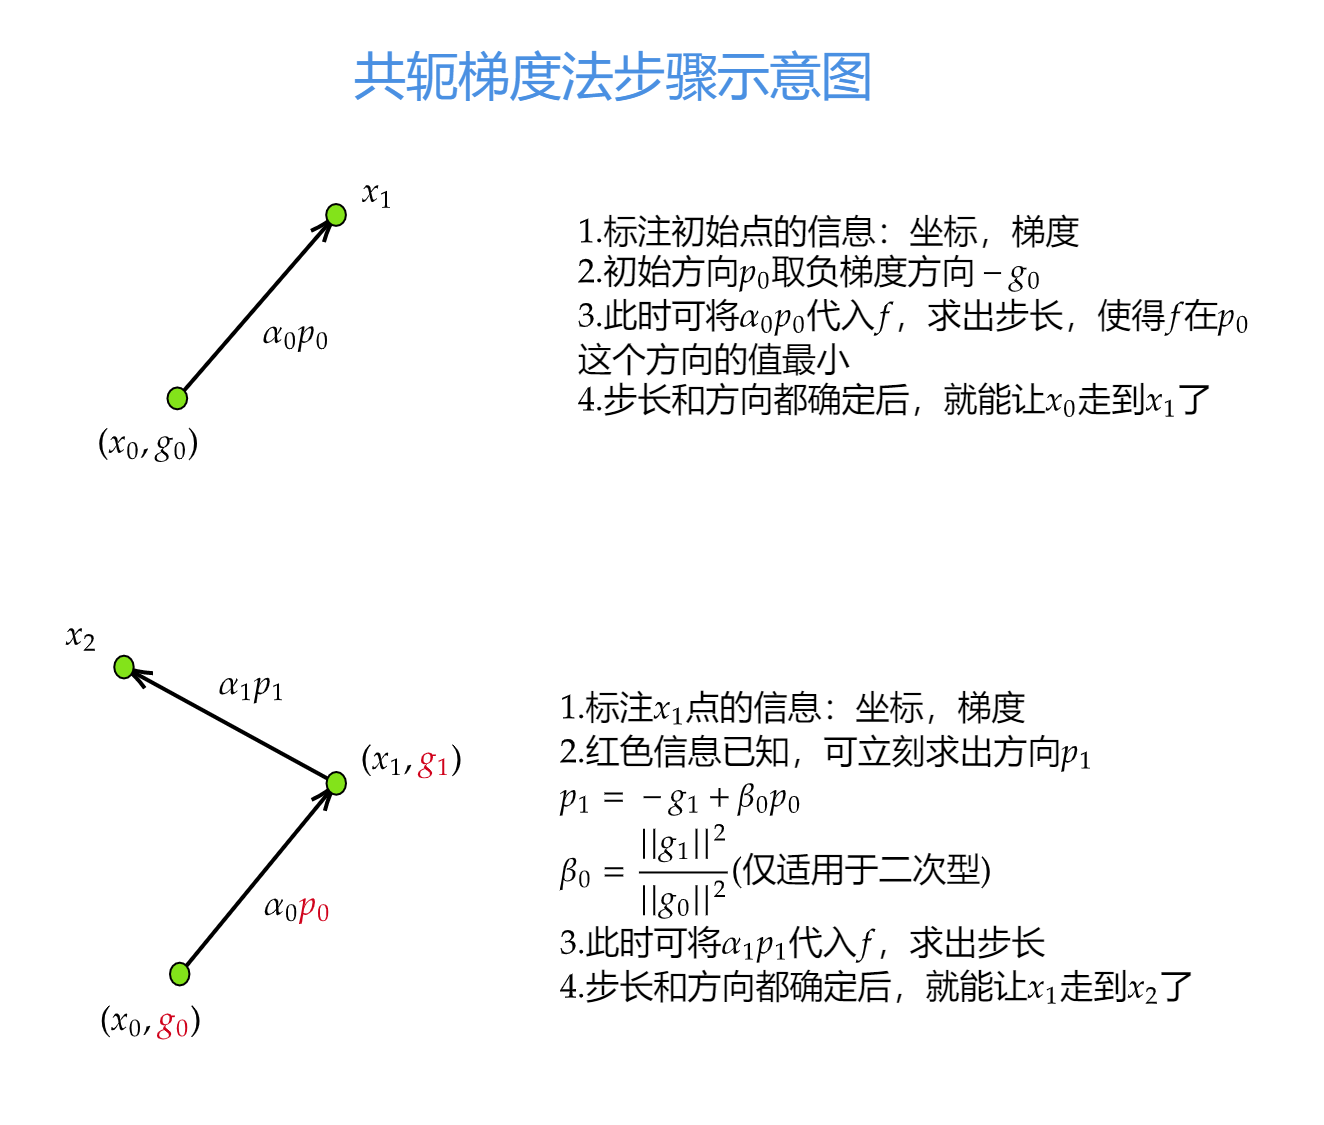
\includegraphics[width=0.8\textwidth]{fig2}
\end{note}
\begin{exercisez}
试用共轭梯度(FR)法求下列问题的最优解:
$$ \mathrm{m}  in  f(x)=x_{1}^{2}+4 x_{2}^{2} ,$$

取初始点为  $x^{(0)}=(4,1)^{T}$ ;
\end{exercisez}
\begin{solution}\\
$\nabla f(x)=g(x)=\left(2 x_{1}, 8 x_{2}\right)^{T}$
\vspace{10pt}

 \textcolor[rgb]{1.00,0.00,0.00}{\large 初始点信息:}
 $ x^{(0)}=(4,1)^{T}, g_{0}=(8,8)^T.$
 \vspace{6pt}

 \textcolor[rgb]{1.00,0.00,0.00}{\large 确定方向$p_0$:}
 $ p_0=-g_{0}=(-8,-8)^T.$
  \vspace{6pt}

 \textcolor[rgb]{1.00,0.00,0.00}{\large 确定步长$\alpha_0$:}
 $ f(x^{(0)}+\alpha_0p_0)=(4-8\alpha_0)^2+4(1-8\alpha_0)^2,$令$f'(\alpha_0)=0,$得$\alpha_0=\frac{1}{5}$.
  \vspace{6pt}

 \textcolor[rgb]{1.00,0.00,0.00}{\large 走向下一点$x^{(1)}$:}
 $ x^{(1)}=x^{(0)}+\alpha_0p_0=(\frac{12}{5},-\frac{3}{5})^T.$
 \vspace{30pt}

 \textcolor[rgb]{0.00,0.50,1.00}{\large 新点$x^{(1)}$的信息:}$x^{(1)}=(\frac{12}{5},-\frac{3}{5})^T,g_{1}=(\frac{24}{5},-\frac{24}{5})^T$
 \vspace{6pt}

 \textcolor[rgb]{0.00,0.50,1.00}{\large 确定方向$p_1$:}
 $ p_1=-g_1+\beta_0p_0=-g_1+\frac{||g_1||^2}{||g_0||^2} p_0=\frac{48}{5}(-4,1)^T$,因为就是一个方向,所以取$p_1=(-4,1)^T$.
  \vspace{6pt}

 \textcolor[rgb]{0.00,0.50,1.00}{\large 确定步长$\alpha_1$:}
 $ f(x^{(1)}+\alpha_1p_1)=\left(2.4-4 \alpha_{1}\right)^{2}+4\left(-0.6+\alpha_{1}\right)^{2},$令$f'(\alpha_1)=0,$得$\alpha_1=0.6$.
  \vspace{6pt}

\textcolor[rgb]{0.00,0.50,1.00}{\large 走向下一点$x^{(2)}$:}
 $ x^{(2)}=x^{(1)}+\alpha_1p_1=(0,0)^T$,顺便求出梯度:$g_2=(0,0)^T$\\
 所以,$X^{*}=(0,0), \min f\left(X^{*}\right)=0.$


\end{solution}

\begin{exercisez}
试用共轭梯度(FR)法求下列问题的最优解:
 $$\min f(X)=2 x_{1}^{2}+x_{2}^{2}+2 x_{1} x_{2}+x_{1}-x_{2} ,$$

 $ \text{取初始点为}  X^{(0)}=(0,0)^{T} .$

\end{exercisez}
\begin{solution}
步骤同上.
\end{solution}





\newpage
\begin{center}
 \textcolor[rgb]{0.33,0.33,1.00}{\huge \bf{4.KT条件}}
\end{center}

\begin{theorem}
  对于一般约束最优化问题:
$$
\begin{aligned}
\min f(\boldsymbol{x}), \boldsymbol{x} & \in \mathbf{R}^{n}, & \\
\text { s.t. } & c_{i}(\boldsymbol{x}) &=0, \quad i \in E=\{1, \cdots, l\}, \\
& c_{i}(\boldsymbol{x}) & \geqslant 0, \quad i \in I=\{l+1, \cdots, m\}
\end{aligned}
$$
 若\\
(i)  $x^{*}$  为局部最优解, 其有效集 $ I^{*}=\left\{i \mid c_{i}\left(x^{*}\right)=0, i \in I\right\}$ ;\\
(ii)  $f(\boldsymbol{x}), c_{i}(\boldsymbol{x})(i=1, \cdots, m)$  在点$  \boldsymbol{x}^{*}  $可微;\\
(iii) 对所有 $ i \in E \cup I^{*}, \nabla c_{i}\left(x^{*}\right)$  线性无关.\\
则存在向量  $\lambda^{*}=\left(\lambda_{1}^{*}, \cdots, \lambda_{m}^{*}\right)^{\mathrm{T}}$  使得
$$
\begin{array}{l}\displaystyle
\nabla f\left(x^{*}\right)-\sum_{i=1}^{m} \lambda_{i}^{*} \nabla c_{i}\left(x^{*}\right)=0, \\
\lambda_{i}^{*} c_{i}\left(x^{*}\right)=0,\lambda_{i}^{*} \geqslant 0, \quad i \in I , \\
c_{i}\left(x^{*}\right)=0,\quad i \in E .
\end{array}
$$
\end{theorem}
\begin{exercisez}
 求解下列约束问题:
$$
\begin{array}{l}
\min f(x)=\left(x_{1}-x_{2}+x_{3}\right)^{2} \\
\text { st. }\left\{\begin{array}{l}
c_{1}(x)=x_{1}+2 x_{2}-x_{3}=5 \\
c_{2}(x)=x_{1}-x_{2}-x_{3}=-1
\end{array}\right.
\end{array}
$$

(1) 写出  $\mathrm{K}-\mathrm{T}$  条件;

(2) 求出$  \mathrm{K}-\mathrm{T} $ 点, 最优解和最优值.
\end{exercisez}
\begin{solution}
...
\end{solution}

\begin{exercisez}
求解下列约束最优化问题:
$$
\begin{array}{l}
\min f(X)=x_{1}^{2}+x_{2}^{2}+x_{3}^{2} \\
\text { s.t. }\left\{\begin{array}{l}
c_{1}(X)=x_{1}+2 x_{2}-x_{3}-4=0, \\
c_{2}(X)=x_{1}-x_{2}-x_{3}+2=0 ;
\end{array}\right.
\end{array}
$$

(1) 写出  $\mathrm{K}-\mathrm{T}  $条件;

(2) 求出 $ \mathrm{K}-\mathrm{T} $ 点, 最优解和最优值.
\end{exercisez}
\begin{solution}
...
\end{solution}




\newpage
\begin{center}
 \textcolor[rgb]{0.33,0.33,1.00}{\huge \bf{5.罚函数法}}
\end{center}

\begin{algorithm}
\begin{center}
  \Large 外罚函数法
\end{center}
对于约束问题 :
$$
\begin{array}{ll}
\min f(\boldsymbol{x}), \boldsymbol{x} \in \mathbf{R}^{n}, & \\
\text { s.t. } & c_{i}(\boldsymbol{x})=0, \quad i \in E=\{1,2, \cdots, l\} \\
& c_{i}(\boldsymbol{x}) \geqslant 0, \quad i \in I=\{l+1, \cdots, m\}
\end{array}
$$
取控制误差 $ \varepsilon>0  $和罚因子的放大系数$  c>1 $ (可取  $\varepsilon=10^{-4}, c=10 $ ).

Step 1 给定初始点  $x_{0}$  (可以不是可行点) 和初始罚因子  $\sigma_{1} $ (可取  $\sigma_{1}=1 $ ), 令 $ k=1$ .\\
Step 2 以  $x_{k-1}$  为初始点求无约束问题:
$$
\min P\left(x, \sigma_{k}\right)=f(x)+\sigma_{k} \tilde{P}(x),
$$
其中 $$
\tilde{\boldsymbol{P}}(\boldsymbol{x})=\sum_{i=1}^{l}\left|c_{i}(\boldsymbol{x})\right|^{\beta}+\sum_{j=l+1}^{m}\left|\min \left(0, c_{j}(\boldsymbol{x})\right)\right|^{\alpha}, \quad\alpha \geqslant 1, \beta \geqslant 1,$$  得最优解  $\boldsymbol{x}_{k}=\boldsymbol{x}\left(\sigma_{k}\right) $.\\
Step 3 若 $ \sigma_{k} \tilde{P}\left(x_{k}\right)<\varepsilon $, 则以$  x_{k}$  为近似最优解, 停止. 否则令$  \sigma_{k+1}=c \sigma_{k}, k=k+1,$ 转 Step 2 .
\end{algorithm}
\begin{note}\\
1.这种方法就是给目标函数$f(x)$加一个惩罚项$ \tilde{P}(x)$,变成增广目标函数$P(x)$.使原目标函数在可行域内不受惩罚,在违反约束的地方受到惩罚(理想情况为$\infty$),其几何解释之前在群聊天里发过,不记得可以翻记录,那里讲的非常清楚.\\
2.直接求$P(x)$的无约束极值即可.\\
\end{note}
\begin{exercisez}
求解约束问题$$
\begin{array}{l}
\min f(x)=x_{1}^{2}+x_{2}^{2} \\
\text { s.t. } x_{1}+1 \leq 0
\end{array}$$
\end{exercisez}
\begin{solution}
令$$\begin{aligned}
P(x, \sigma)
&=\left\{\begin{array}{ll}
x_{1}^{2}+x_{2}^{2}, & x_{1}+1 \leq 0 \\
x_{1}^{2}+x_{2}^{2}+\sigma\left(x_{1}+1\right)^{2}, & x_{1}+1>0
\end{array}\right.
\end{aligned}$$
令$\begin{cases}
   \frac{\partial P}{\partial x_1}=0 \\
   \frac{\partial P}{\partial x_2}=0
 \end{cases}$

当$x_1\leq -1 $时,
  $\begin{cases}
\frac{\partial P}{\partial x_1}=2x_1,   \\
\frac{\partial P}{\partial x_2}=2x_2,
\end{cases}$,解得$(x_1,x_2)=(0,0),$舍去;

当$x_1>-1$时,
$\begin{cases}
\frac{\partial P}{\partial x_1}=2x_1+2\sigma (x_1+1) \\
\frac{\partial P}{\partial x_2}=2x_2,
\end{cases}$,解得$(x_1,x_2)=(-\frac{\sigma}{\sigma+1},0),$

它是$P(x, \sigma)$的最优点,最优值为$P(x, \sigma)=\frac{\sigma}{\sigma+1}$.

当  $\sigma \rightarrow+\infty$  时,  $x_{1}(\sigma) \rightarrow-1, x_{2}(\sigma) \rightarrow 0 .$
因此 $ x(\sigma) \rightarrow x^{*}, P(x, \sigma) \rightarrow f\left(x^{*}\right)=1 .$

\begin{remark}
一般题目约束是起作用的,所以不必求没有惩罚的那一段函数的极值.
\end{remark}

\end{solution}

\newpage
\begin{exercisez}
求解约束问题$$
\begin{array}{l}
\min f(x)=x_{1}^{2}+x_{2}^{2} \\
\text { s.t. } x_{1}+1 = 0
\end{array}$$
\end{exercisez}
\begin{solution}
令$$\begin{aligned}
P(x, \sigma)
&=\left\{\begin{array}{ll}
x_{1}^{2}+x_{2}^{2}, & x_{1}+1 = 0 ,\\
x_{1}^{2}+x_{2}^{2}+\sigma\left(x_{1}+1\right)^{2}, & x_{1}+1\neq 0,
\end{array}\right.
\end{aligned}=x_{1}^{2}+x_{2}^{2}+\sigma\left(x_{1}+1\right)^{2}$$
令$\begin{cases}
   \frac{\partial P}{\partial x_1}=0 \\
   \frac{\partial P}{\partial x_2}=0
 \end{cases}$,
$\begin{cases}
\frac{\partial P}{\partial x_1}=2x_1+2\sigma (x_1+1) \\
\frac{\partial P}{\partial x_2}=2x_2,
\end{cases}$,解得$(x_1,x_2)=(-\frac{\sigma}{\sigma+1},0),$

它是$P(x, \sigma)$的最优点,最优值为$P(x, \sigma)=\frac{\sigma}{\sigma+1}$.

当  $\sigma \rightarrow+\infty$  时,  $x_{1}(\sigma) \rightarrow-1, x_{2}(\sigma) \rightarrow 0 .$
因此 $ x(\sigma) \rightarrow x^{*}, P(x, \sigma) \rightarrow f\left(x^{*}\right)=1 .$

\end{solution}
\begin{exercisez}
 求解约束问题:
$$
\begin{array}{l}
\min f(x)=x_{1}^{2}+x_{1} x_{2}+x_{2}^{2}, \\
\text { s.t. } c(x)=x_{1}+x_{2}-2=0
\end{array}
$$
\end{exercisez}
\begin{solution}
\quad 这道题就是后面的乘子法的试题,这里先用外罚函数法写一写,后面的乘子法求解步骤类似.考试的话只考其一,最近两次考的都是乘子法.
\end{solution}
\vspace{18pt}

\begin{note}
\begin{center}
  \textcolor[rgb]{0.33,0.33,1.00}{\Large 计算机求解思路}
\end{center}
构造一堆增广函数,惩罚项系数按一定的倍数增加,分别用无约束算法求解每个增广函数的极值点
\vspace{10pt}

以上上题为例,大致步骤如下(惩罚系数$\sigma$的增大倍数设为10):
\vspace{7pt}

1.给定初始点$x_0$,增广目标函数$P(x, \sigma_1)=P(x, 0.1)=x_{1}^{2}+x_{2}^{2}+0.1\left(x_{1}+1\right)^{2}$,
用牛顿法或者别的无约束算法求得$P(x, \sigma_1)$的最优点,记为$x_1$.

2.将$x_1$视为新的初始点,增广目标函数$P(x, \sigma_2)=P(x, 1)=x_{1}^{2}+x_{2}^{2}+\left(x_{1}+1\right)^{2}$,
用牛顿法或者别的无约束算法求得$P(x, \sigma_2)$的最优点,记为$x_2$.

3.将$x_2$视为新的初始点,增广目标函数$P(x, \sigma_3)=P(x, 10)=x_{1}^{2}+x_{2}^{2}+10\left(x_{1}+1\right)^{2}$,
用牛顿法或者别的无约束算法求得$P(x, \sigma_3)$的最优点,记为$x_3$.
\vspace{7pt}

终止条件:$ \sigma_{k} \tilde{P}\left(x_{k}\right)<\varepsilon $ \quad \quad 因为KT条件没法直接拿来用,这里是因为$\{x_k\}$收敛时,$  \sigma_{k} \tilde{P}\left(x_{k}\right) \rightarrow 0 $

\centerline{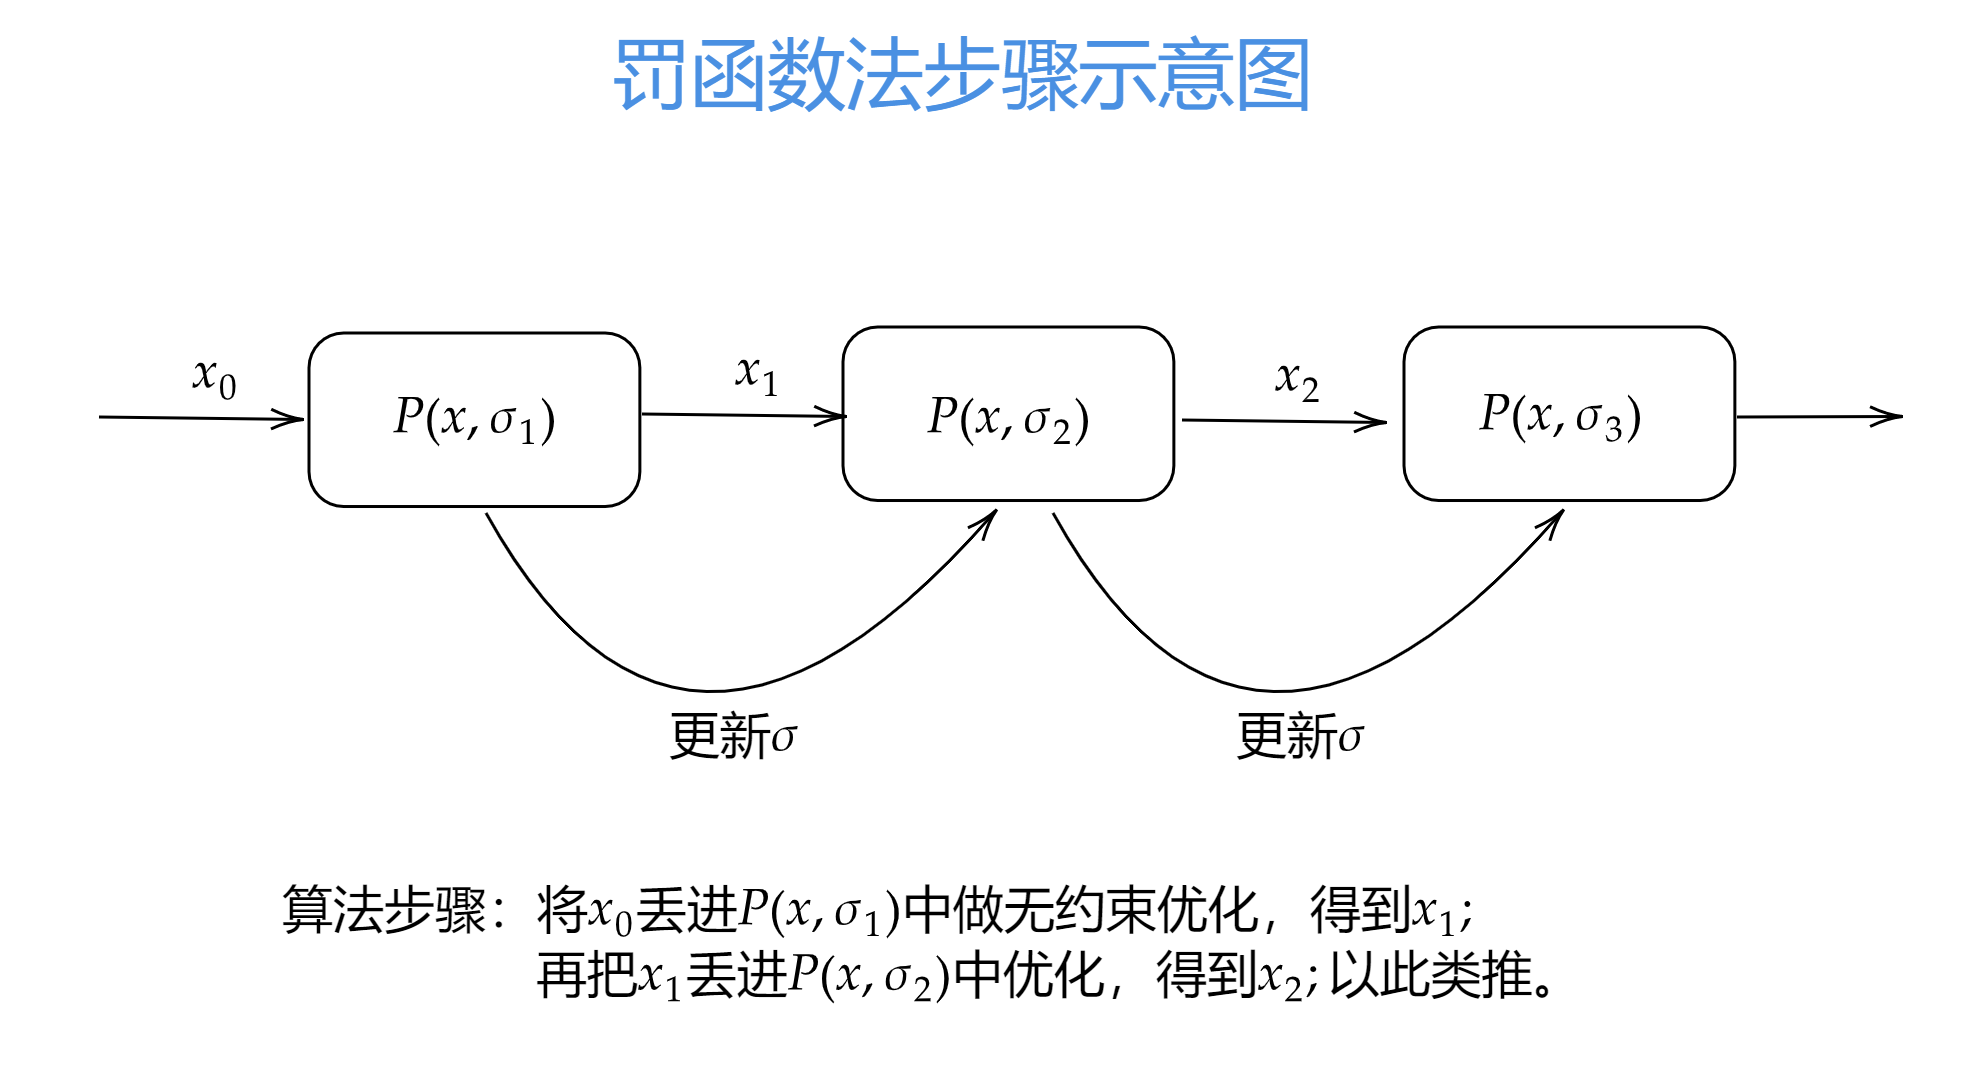
\includegraphics[width=0.8\textwidth]{fig3}}

\end{note}
\newpage
\begin{algorithm}
\begin{center}
  \Large 内罚函数法
\end{center}
求解约束问题
$$\begin{array}{c}
    \min f(x), \quad x \in \mathbf{R}^{n}
 \\
    s.t.  \quad c_{i}(x) \geqslant 0, \quad i=1, \cdots, m
  \end{array} $$
 且其可行域的内点集 $ D_{0} \neq \varnothing .$\\
构造如下的增广目标函数:
$$
B(x, r)=f(x)+r \tilde{B}(x),
$$
其中令
$$
\tilde{B}(\boldsymbol{x})=\sum_{i=1}^{m} \frac{1}{c_{i}(\boldsymbol{x})} \text { 或 } \tilde{B}(\boldsymbol{x})=-\sum_{i=1}^{m} \ln \left(c_{i}(\boldsymbol{x})\right) \text {, }
$$
取控制误差  $\varepsilon>0 $ 和罚因子的缩小系数 $ 0<c<1  $(可取  $\varepsilon=10^{-4}, c=0.1$  ).\\
Step 1 选定初始点 $ x_{0} \in D_{0}$ , 给定  $r_{1}>0\left(\right. $ 取  $r_{1}=10 $ ), 令 $ k=1 $.\\
Step 2 以  $x_{k-1}$  为初始点, 求解无约束问题
$$
\min B\left(x, r_{k}\right)=f(x)+r_{k} \tilde{B}(x),
$$
 得最优解  $\boldsymbol{x}_{k}=\boldsymbol{x}\left(r_{k}\right) $.\\
Step 3 若 $ r_{k} \tilde{B}\left(x_{k}\right)<\varepsilon $, 则 $ \boldsymbol{x}_{k} $ 为 近似最优解, 停. 否则, 令$  r_{k+1}=c r_{k}, k=k+1$  转 Step  2 .
\end{algorithm}


\begin{exercisez}
(非数学专业必答) 请用内点法求解下列问题:
$$
\begin{array}{l}
\min f(X)=\frac{1}{6}\left(x_{1}+1\right)^{3}+x_{2}-1 \\
\text { s.t. }\left\{\begin{array}{l}
c_{1}(X)=x_{1}-1 \geq 0 \\
c_{2}(X)=x_{2}-1 \geq 0
\end{array}\right.
\end{array}
$$

(1)推导其最优解;

(2) 若取  $X_{0}=(3,5), r_{1}=2 $, 公比 $ c=\frac{1}{2}$  时,指出用何种方法可计算点列  $X_{1}, X_{2}, \cdots, X_{k}, \cdots ;$
\end{exercisez}
\begin{solution}
...
\end{solution}




\newpage
\begin{center}
 \textcolor[rgb]{0.33,0.33,1.00}{\huge \bf{6.乘子法}}
\end{center}

\begin{algorithm}
\begin{center}
  \Large 等式约束问题的乘子法(  $\mathrm{PH}$  算法)
\end{center}

Step 1 选定初始点 $ x_{0}$  ,初始乘子向量$  \lambda_{1}$  ,初始罚因子  $\sigma_{1}$  及其放 大系数$  c>1 $ ,控制误差 $ \varepsilon>0$  与常数  $\theta \in(0,1)$ , 令  $k=1$ .\\
Step 2 以  $x_{k-1} $ 为初始点求解无约束问题
$$
\min M\left(\boldsymbol{x}, \lambda_{k}, \sigma_{k}\right)=f(\boldsymbol{x})-\lambda_{k}{ }^{\mathrm{T}} \boldsymbol{c}(\boldsymbol{x})+\frac{\sigma_{k}}{2} \boldsymbol{c}(\boldsymbol{x})^{\mathrm{T}} \boldsymbol{c}(\boldsymbol{x})
$$
得最优解  $\boldsymbol{x}_{k} $.\\
Step 3 当 $ \left\|\boldsymbol{c}\left(x_{k}\right)\right\|<\varepsilon  $时,  $x_{k} $ 为所求最优解, 停. 否则转Step 4 .\\
Step 4 当  $\left\|c\left(x_{k}\right)\right\| /\left\|c\left(x_{k-1}\right)\right\| \leqslant \theta $ 时, 转 Step 5 , 否则令 $ \sigma_{k+1}=c \sigma_{k}$ , 转 Step 5 .\\
 Step 5 令 $\lambda_{k+1}=\lambda_{k}-\sigma_{k} c\left(x_{k}\right), k=k+1 , $转 Step  2 .
\end{algorithm}
\begin{note}
\begin{center}
  \textcolor[rgb]{0.00,0.00,1.00}{\Large 算法设计思路(不清楚在讲啥可跳过)}
\end{center}

原始形式的外罚函数法存在一个严重的缺点,就是$\sigma$必须趋于无穷大,才能让点列收敛到最优点,但是这样的增广函数性质很垃圾,梯度差的一比,很难优化。而拉格朗日函数虽然可以直接使用无约束优化算法,但是有的情况下这个拉格朗日函数不存在极值点,其稳定点是个鞍点,无约束算法不一定能走到这个鞍点上来。

解决方案:对拉格朗日函数再进行约束,使它变成约束问题,并且这个约束问题与原始约束问题等价。对这个拉格朗日函数进行外罚函数法。

由于带约束的拉格朗日函数,在最优点处,其Hessian矩阵一定在约束可行域内正定,由Finsler定理(教材P158)可以证明,一定存在一个数$\sigma^*>0$,使得当$\sigma\geq\sigma^*$时,对于整个空间,都有$\nabla_{x}^{2} L\left(x^{*}, \lambda^{*}\right)+\sigma \nabla \boldsymbol{A}\left(x^{*}\right) \boldsymbol{A}\left(x^{*}\right)^{\mathrm{T}}$正定,其中$ \nabla \boldsymbol{A}\left(x^{*}\right) \boldsymbol{A}\left(x^{*}\right)^{\mathrm{T}}$是罚函数$ \tilde{P}(x)=\frac{1}{2} \boldsymbol{c}(\boldsymbol{x})^{\mathrm{T}} \boldsymbol{c}(\boldsymbol{x})$的二阶导.

而$\nabla_{x}^{2} L\left(x^{*}, \lambda^{*}\right)+\sigma \nabla \boldsymbol{A}\left(x^{*}\right) \boldsymbol{A}\left(x^{*}\right)^{\mathrm{T}}$是如下函数(增广拉格朗日函数)的Hessian矩阵:
$$M(x, \lambda, \sigma)=L(x, \lambda)+\frac{\sigma}{2} c(x)^{\mathrm{T}} c(x)$$

说明了上述条件下,在最优点处,拉格朗日增广函数在全空间内都是正定的,就能用无约束优化算法,并且梯度性质较好.

\centerline{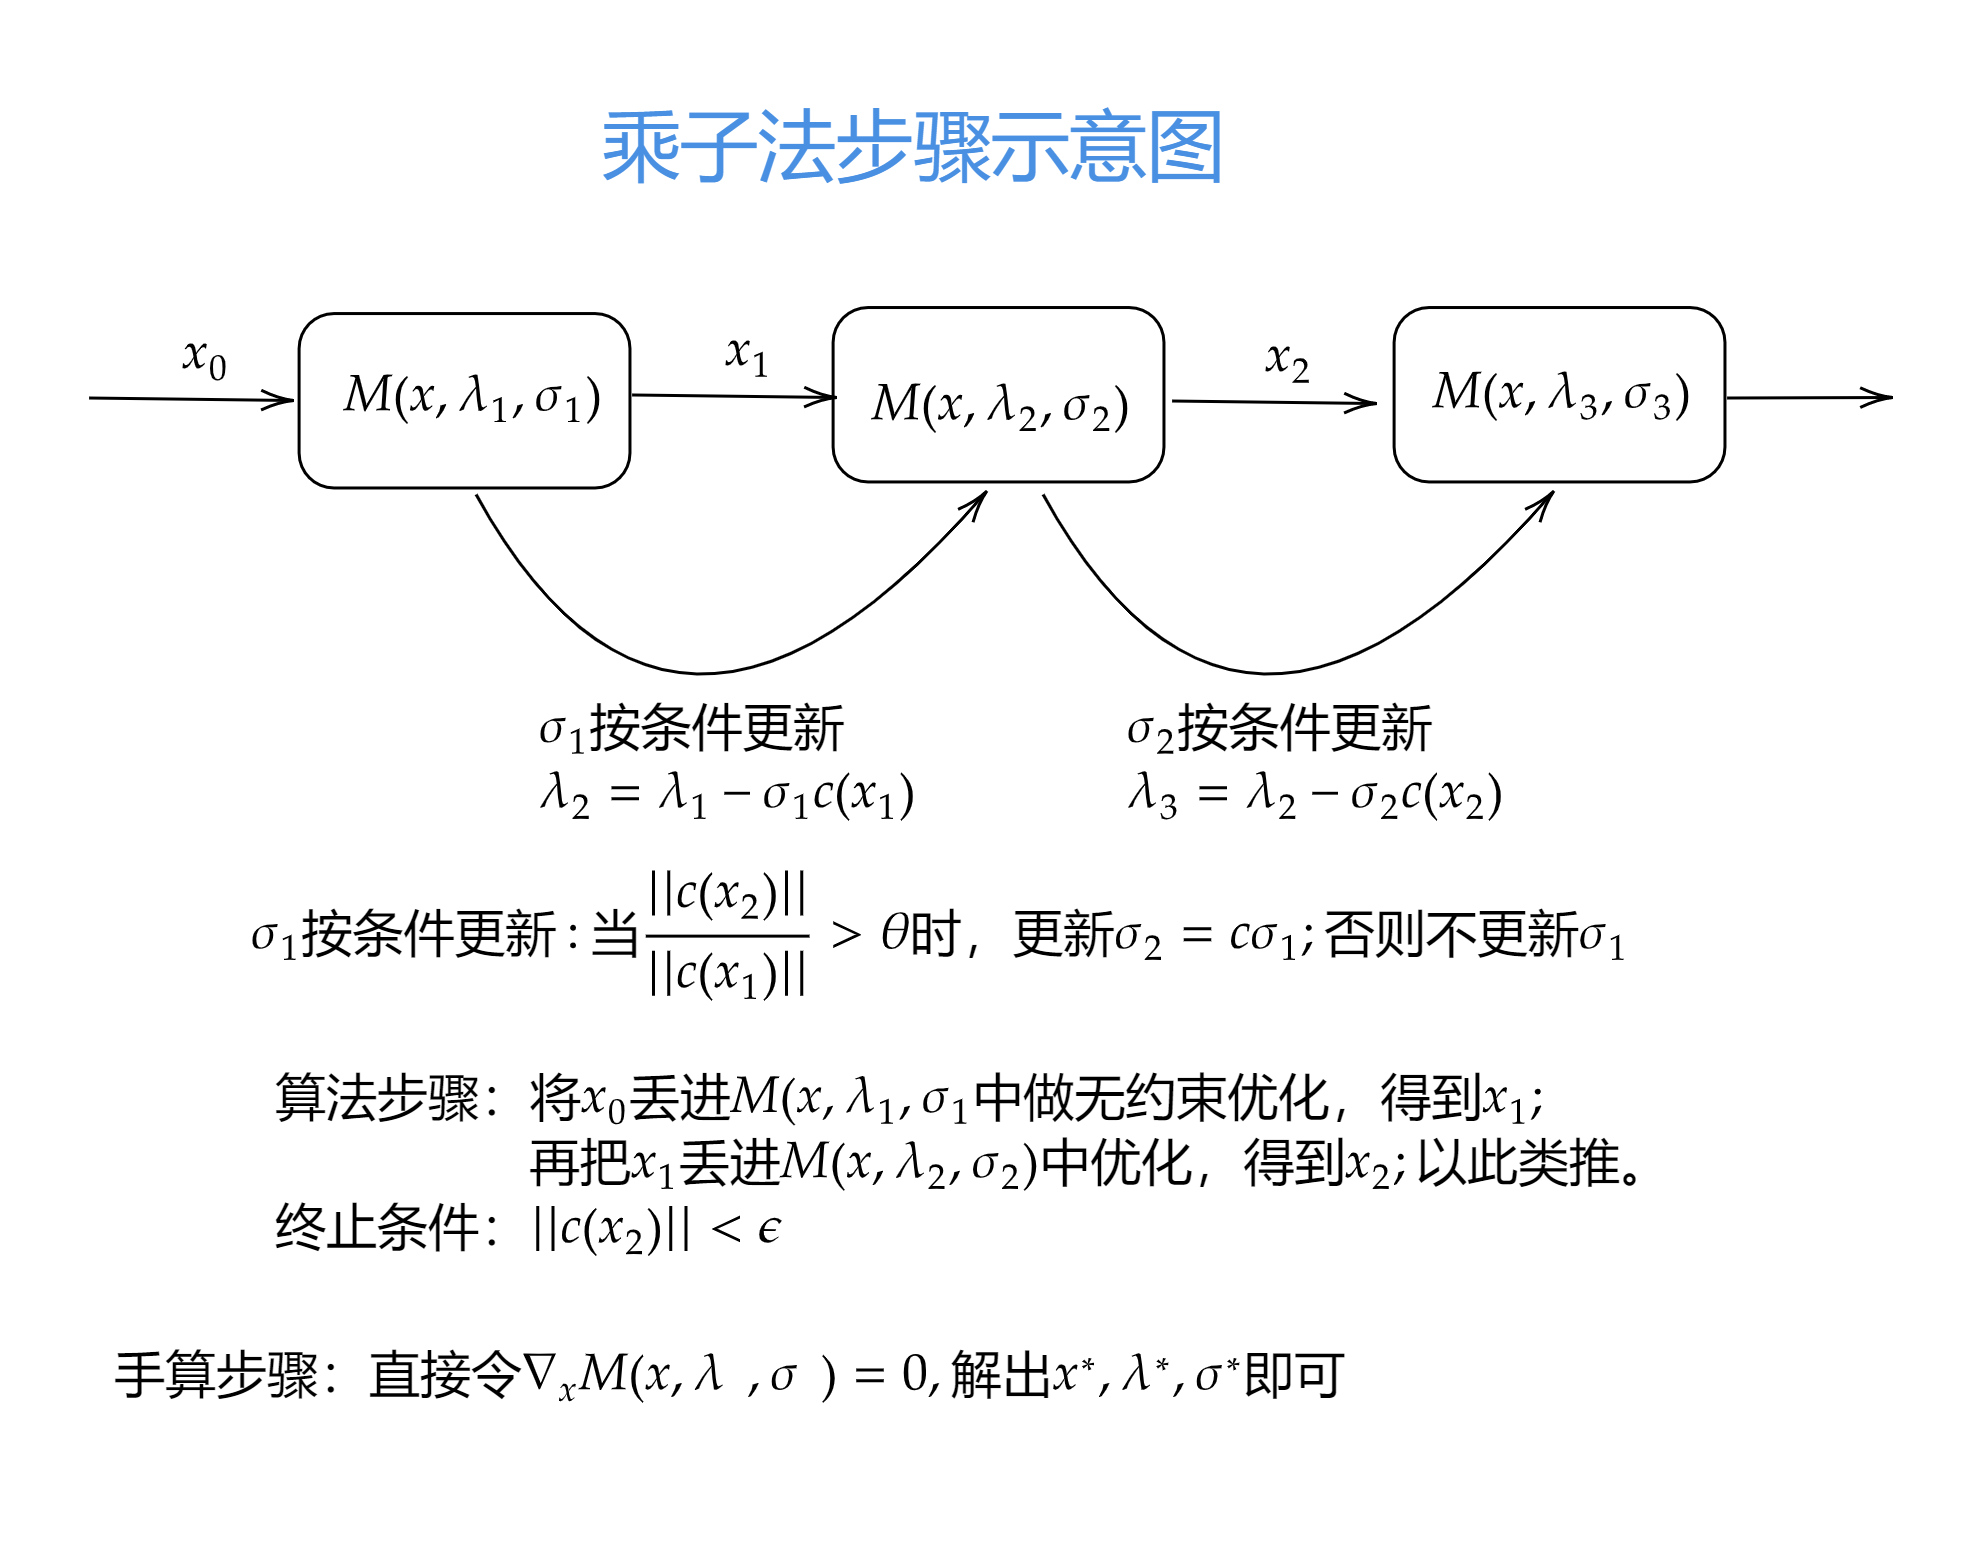
\includegraphics[width=0.8\textwidth]{fig4}}
\end{note}
\begin{exercisez}
 试用乘子法求下列问題的最优解:
$$
\begin{array}{l}
\min f(x)=x_{1}^{2}+x_{1} x_{2}+x_{2}^{2}, \\
\text { s.t. } c(x)=x_{1}+x_{2}-2=0
\end{array}
$$
\end{exercisez}
\begin{solution}\\

增广 Lagrange 函数为:  $$M(\boldsymbol{x}, \lambda, \sigma)=\frac{1}{2} \boldsymbol{x}^{T} \boldsymbol{G} \boldsymbol{x}-\lambda\left(x_{1}+x_{2}-2\right)+\frac{\sigma}{2}\left(x_{1}+x_{2}-2\right)^{2}, \sigma>0 ,$$
令$$ \nabla M(x, \lambda, \sigma)=\boldsymbol{G} \boldsymbol{x}-\lambda \nabla c(\boldsymbol{x})+\sigma c(\boldsymbol{x}) \nabla c(\boldsymbol{x})=0$$
其中 $$\nabla c(\boldsymbol{x})=\left(\begin{array}{l}1 \\ 1\end{array}\right), \lambda \nabla c(\boldsymbol{x})=\lambda\left(\begin{array}{l}1 \\ 1\end{array}\right), \sigma \nabla c(\boldsymbol{x}) \cdot c(\boldsymbol{x})=\sigma\left(\begin{array}{l}1 \\ 1\end{array}\right)(1,1) \boldsymbol{x}-2 \sigma\left(\begin{array}{l}1 \\ 1\end{array}\right)=\sigma\left(\begin{array}{ll}1 & 1 \\ 1 & 1\end{array}\right) \boldsymbol{x}-2 \sigma\left(\begin{array}{l}1 \\ 1\end{array}\right) ,$$
所以,
$$\nabla M(x, \lambda, \sigma)=\left(\begin{array}{ll}
2 & 1 \\
1 & 2
\end{array}\right) x-\lambda\left(\begin{array}{l}
1 \\
1
\end{array}\right)+\sigma\left(\begin{array}{ll}
1 & 1 \\
1 & 1
\end{array}\right) x-2 \sigma\left(\begin{array}{l}
1 \\
1
\end{array}\right)=\left(\begin{array}{ll}
2+\sigma & 1+\sigma \\
1+\sigma & 2+\sigma
\end{array}\right) \left(\begin{array}{ll}
x_1 \\
x_2
\end{array}\right)-\left(\begin{array}{l}
\lambda+2 \sigma \\
\lambda+2 \sigma
\end{array}\right)=0,
$$
解得,
$$
x_{1}=x_{2}=\frac{\lambda+2 \sigma}{3+2 \sigma}\rightarrow 1(\sigma\rightarrow\infty),
$$
故存在$\sigma^*$,使得$\frac{\lambda+2 \sigma^*}{3+2 \sigma^*}=1,$得$\lambda=3$.
因此$$x^*=(1,1)^T,f*=3.$$
\end{solution}
\newpage
\begin{exercisez}
请用乘子法求下列问题的最优解:
$$
\begin{array}{c}
  \min f(x)=x_1^2-3x_2-x_2^2, \\
  \text { s.t. } x_{2}=0 \text {. }
\end{array}
$$

\end{exercisez}
\begin{solution}\\
增广 Lagrange 函数为:$$
M(x, \lambda, \sigma)=x_{1}^{2}-(\lambda+3) x_{2}+\frac{\sigma-2}{2} x_{2}^{2}$$
令 $$ \begin{array}{l}
\frac{\partial M}{\partial x_{1}}=2 x_{1}=0, \\
\frac{\partial M}{\partial x_{2}}=(\sigma-2) x_{2}-(\lambda+3)=0,
\end{array}
$$
得  $\quad x_{0}=\left(0, \frac{\lambda+3}{\sigma-2}\right)^{\mathrm{T}} .$
要求 $ x_{0}$  满足的约束条件 $ x_{2}=0$ , 必须取$  \lambda=-3$ , 从而$  x_{0}=(0,0)^{\mathrm{T}}=x^{*} $, 即为原约束问题的最优解.

\end{solution}

\begin{exercisez}
 (数学专业必答)对上题,已知初始点$  X_{0}$ , 初始乘子向量  $\lambda_{1} $, 初始罚因子$  \sigma_{1} $, 放大 系数  $c>1$ , 控制误差 $ \varepsilon>0 $, 常数 $ \theta \in(0,1) $, 如何求出迭代点列 $ X_{1}, X_{2}, \cdots, X_{k}, \cdots ;$
\end{exercisez}
\begin{solution}\\
就是简要概述一下算法,结合上面给的算法步骤和图片,随便讲讲,注意$\sigma$和$\lambda$的更新,以及终止条件。
\end{solution}




\newpage
\begin{center}
 \textcolor[rgb]{0.33,0.33,1.00}{\huge \bf{7.简约梯度法}}
\end{center}

\begin{algorithm}
需要用到的公式:\\
$1.\quad r\left(x^{N}\right)=\nabla_{N} f\left(x^{B}\left(x^{N}\right), x^{N}\right)-\left(B^{-1} N\right)^{\mathrm{T}} \nabla_{B} f\left(x^{B}\left(x^{N}\right), x^{N}\right)$\\
$2.\quad \left(p_{k}^{N}\right)_{j}=\left\{\begin{array}{ll}
-\left(x_{k}^{N}\right)_{j} r_{j}\left(x_{k}^{N}\right), & \text { 当 } r_{j}\left(x_{k}^{N}\right)>0 \text { 时, } \\
-r_{j}\left(x_{k}^{N}\right), & \text { 当 } r_{j}\left(x_{k}^{N}\right) \leqslant 0 \text { 时. }
\end{array}\right.$\\
$3.\quad \boldsymbol{p}_{k}^{B}=-\boldsymbol{B}^{-1} \boldsymbol{N p}_{k}^{N}$\\
$4.\quad \alpha_{\max }=\left\{\begin{array}{ll}
\min \left\{\frac{\left(\boldsymbol{x}_{k}\right)_{j}}{-\left(\boldsymbol{p}_{k}\right)_{j}} \mid\left(\boldsymbol{p}_{k}\right)_{j}<0\right\}, & \text { 当 } \boldsymbol{p}_{k} \neq \boldsymbol{0} \text { 时, } \\
+\infty, & \text { 当 } \boldsymbol{p}_{k} \geqslant \mathbf{0} \text { 时, }
\end{array}\right.$\\
Step 1 给定初始基可行解 $ x_{1}=\left(\begin{array}{l}x_{1}^{B} \\ x_{1}^{N}\end{array}\right) \geqslant 0 $, 其中 $ x_{1}^{B}$  为基向量, 令 $ k   =1$ .\\
Step 2 对应于$  \boldsymbol{x}_{k}=\left(\begin{array}{l}\boldsymbol{x}_{k}^{B} \\ \boldsymbol{x}_{k}^{N}\end{array}\right) $ 将 $ \boldsymbol{A} $ 分解成  $\boldsymbol{A}=(\boldsymbol{B}, \boldsymbol{N})$ . 由公式 1, 2 和 3 分别计算  $r\left(x_{k}^{N}\right), \boldsymbol{p}_{k}^{N}$  和 $ \boldsymbol{p}_{k}^{B}$ , 令  $\boldsymbol{p}_{k}=\left(\begin{array}{c}\boldsymbol{p}_{k}^{B} \\ \boldsymbol{p}_{k}^{N}\end{array}\right) .$
\\
Step 3 若$  \boldsymbol{p}_{k}=\mathbf{0} $, 则 $ \boldsymbol{x}_{k}$  为 KT 点, 停; 否则, 由式 4 计算$  \alpha_{\max } $, 求  $\alpha_{k}$  使
$$
f\left(\boldsymbol{x}_{k}+\alpha_{k} \boldsymbol{p}_{k}\right)=\min _{0 \leqslant \alpha \leqslant \alpha_{\max }} f\left(\boldsymbol{x}_{k}+\alpha \boldsymbol{p}_{k}\right),
$$
令  $\boldsymbol{x}_{k+1}=\boldsymbol{x}_{k}+\alpha_{k} \boldsymbol{p}_{k}$ , 转 Step 4 .\\
Step 4 若$  \boldsymbol{x}_{k+1}^{B}>0$ , 则基向量不变, 令 $ k=k+1$ , 转 Step 2; 若有某 个  j  使  $\left(\boldsymbol{x}_{k+1}^{B}\right)_{j}=0 $, 则将  $\left(\boldsymbol{x}_{k+1}^{B}\right)_{j}$  换出基, 而以 $ \boldsymbol{x}_{k+1}^{N} $ 中具有最大分量的变 量换入基, 构成新的基向量  $\boldsymbol{x}_{k+1}^{B}  $与非基向量 $ \boldsymbol{x}_{k+1}^{N}$ , 令$  k=k+1$ , 转Step 2 .
\end{algorithm}

\begin{exercisez}
试述简约梯度法的迭代步骤;
\end{exercisez}
\begin{solution}
...
\end{solution}
\begin{exercisez}
试用简约梯度法求出初始点$  X^{(1)} $ 和搜索方向 $ \boldsymbol{p}_{1} $, 以及步长的上限 $ \alpha_{\text {max }} ;$
$$
\begin{array}{l}
\min f(X)=x_{1}^{2}+x_{1} x_{2}+2 x_{2}^{2}-6 x_{1}-14 x_2, \\
\text { s.t. }\left\{\begin{array}{l}
c_{1}(X)=x_{1}+x_{2}+x_{3}=2, \\ c_{2}(X)=-x_{1}+2 x_{2} \quad+x_{4}=3, \\
x_{i}>0, i=1,2,3,4 ;
\end{array}\right.
\end{array}
$$
\end{exercisez}
\begin{solution}
...
\end{solution}


\end{document}










